\section{Results}
    \subsection{Fluxes results}

    \paragraph{22.04.2022 results}
    ???

        \begin{figure}[H]
        \centering
        \begin{subfigure}{\textwidth}
            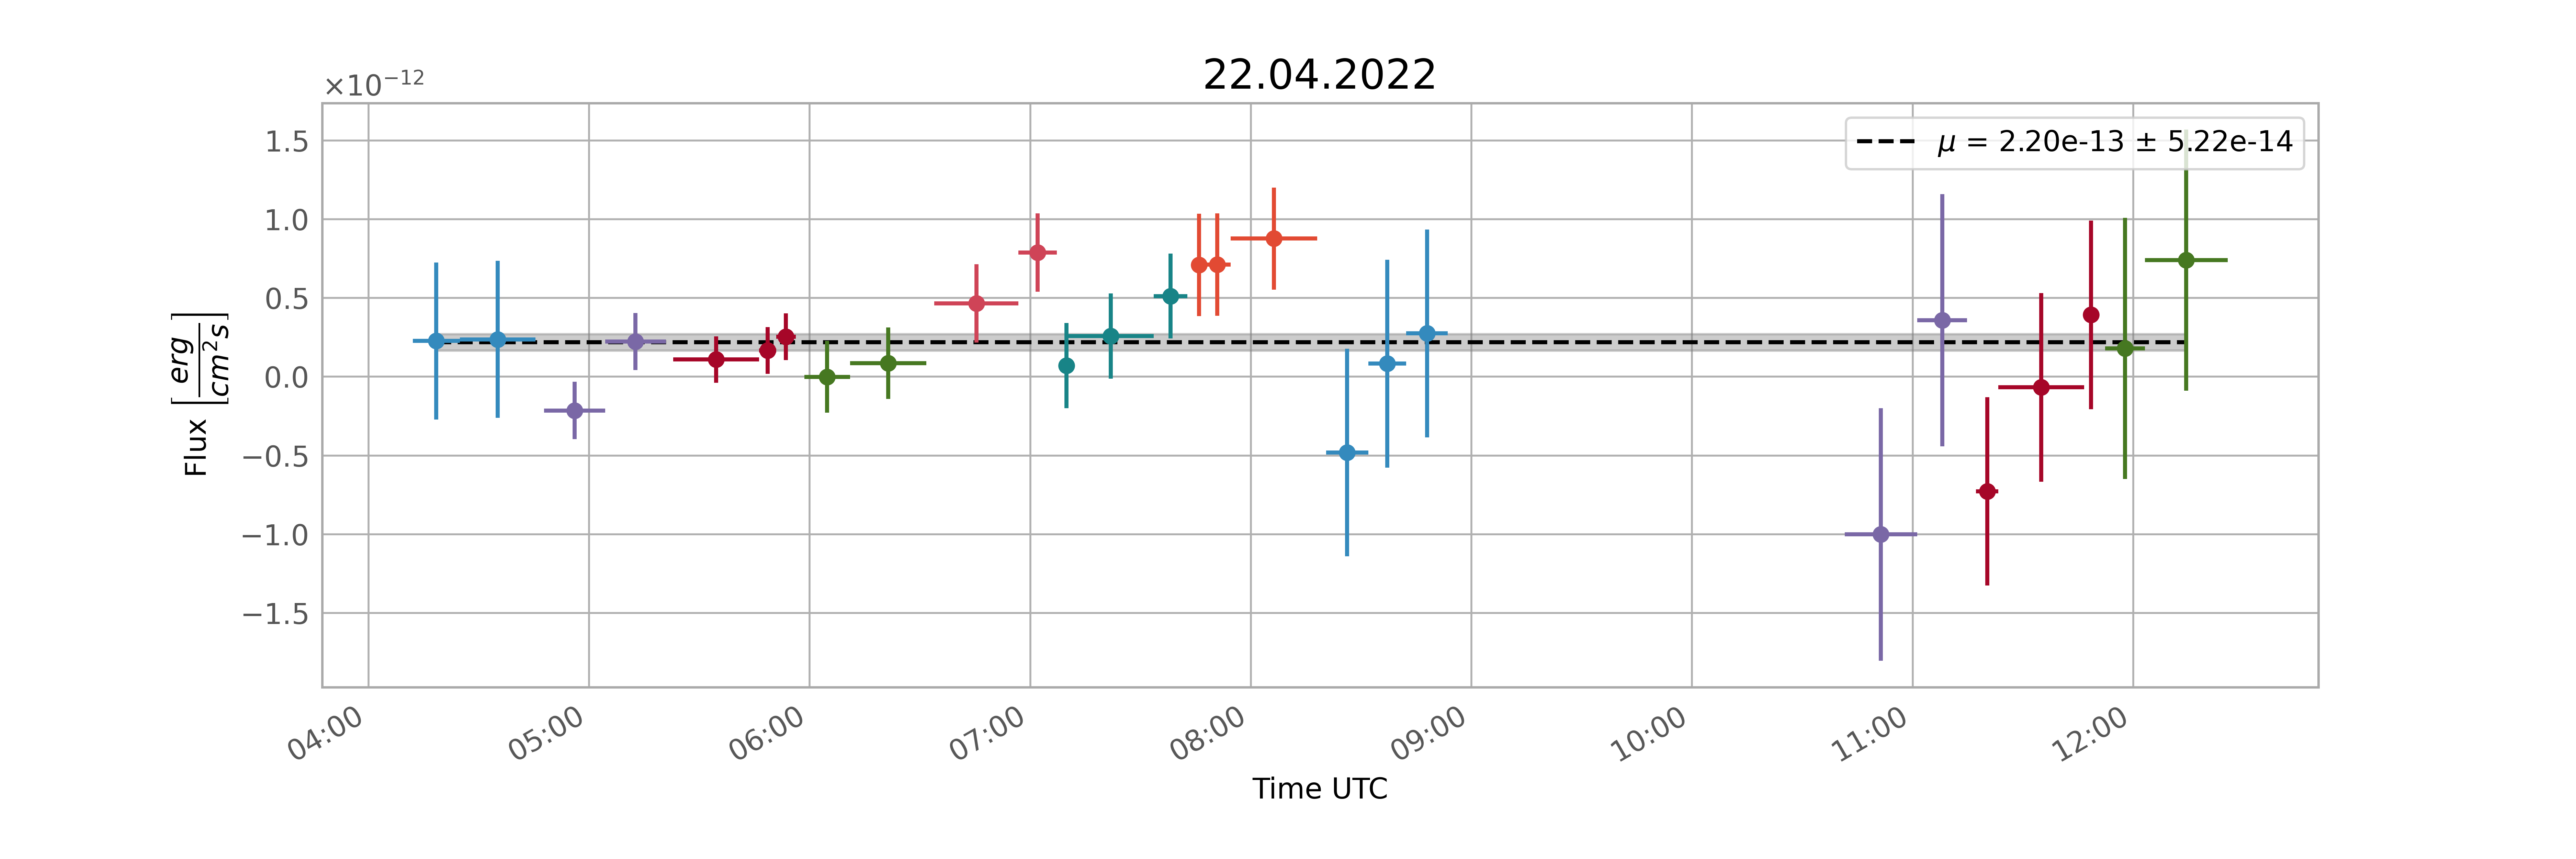
\includegraphics[width=\textwidth]{report/Figures/results/lc_2204.png}
        \end{subfigure}%
        \hspace{1em}
        \begin{subfigure}{\textwidth}
            \centering
            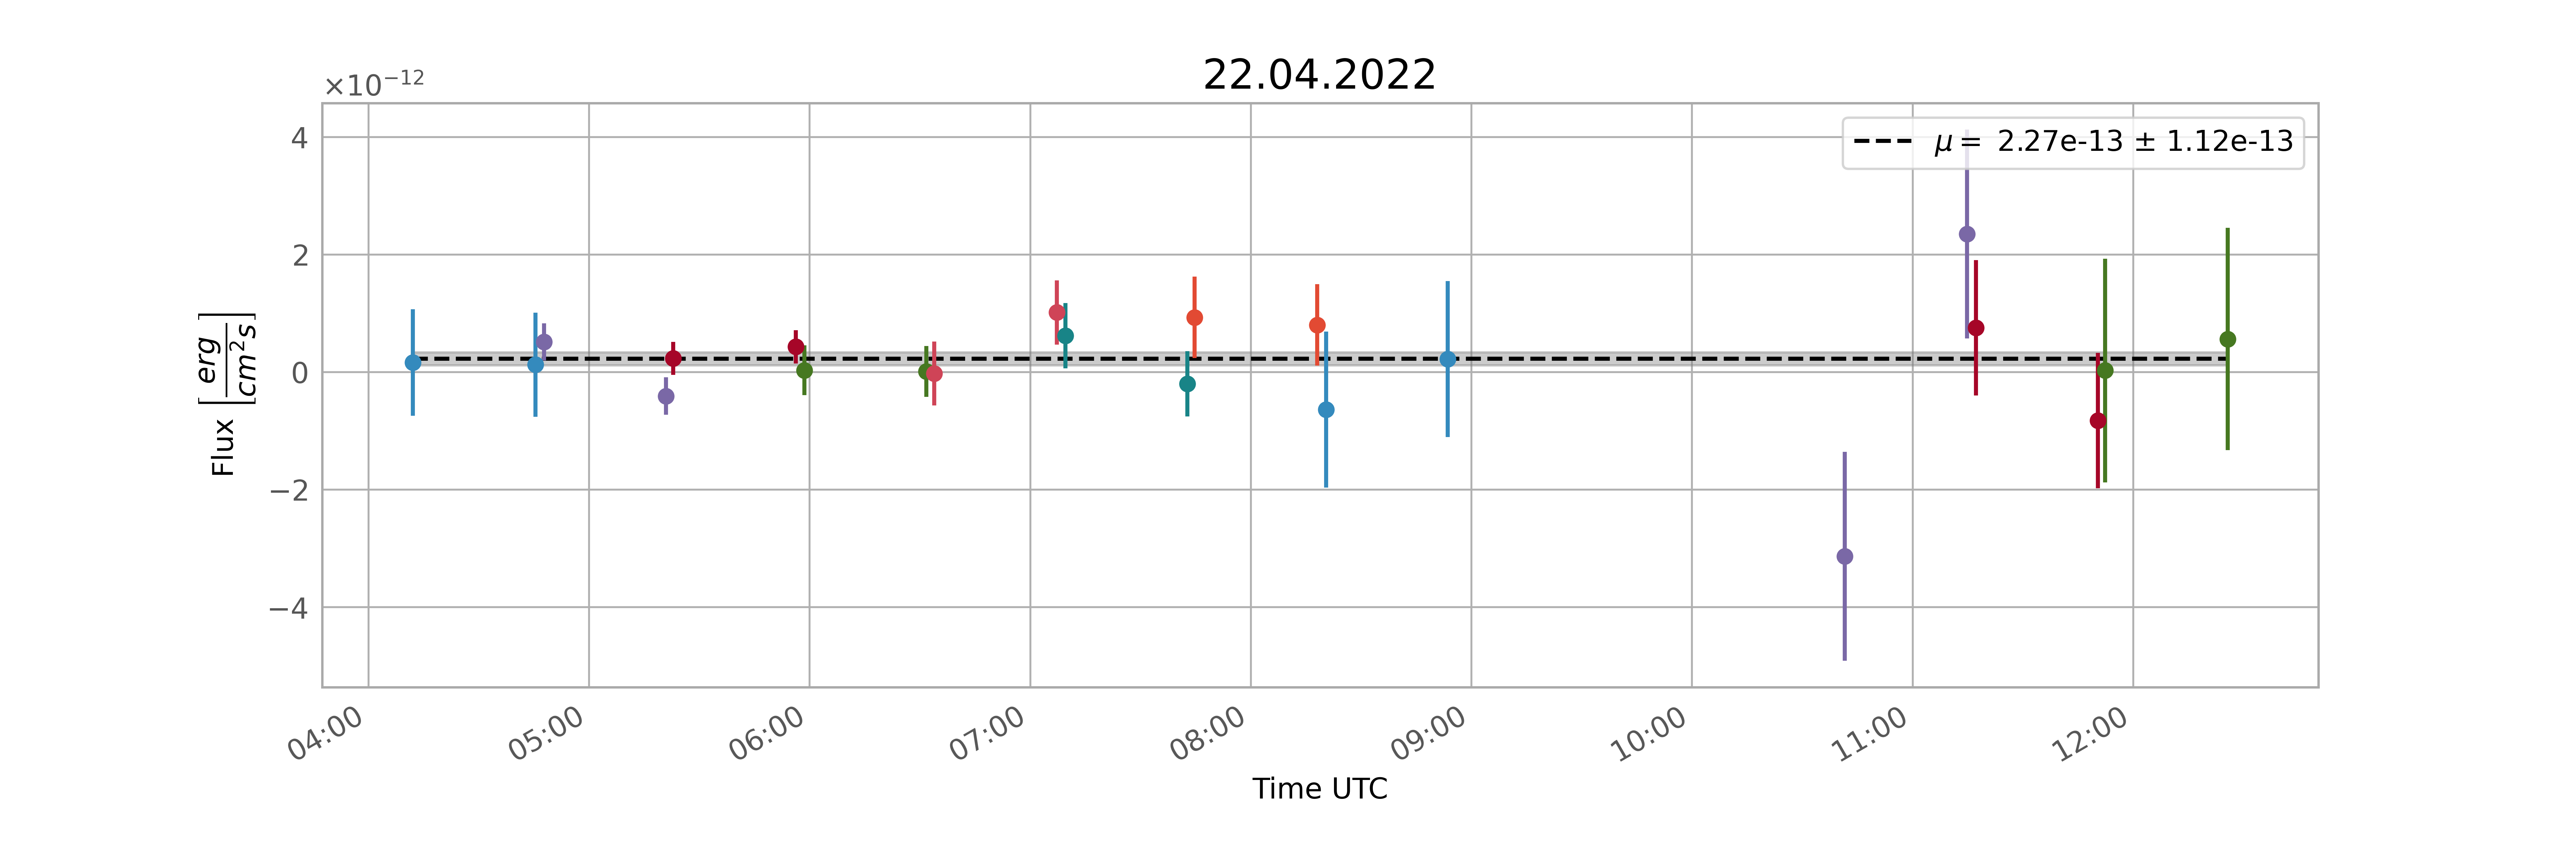
\includegraphics[width=\textwidth]{report/Figures/results/lc_2204_psf_notconst.png}
        \end{subfigure}
        \hspace{1em}
        \begin{subfigure}{\textwidth}
            \centering
            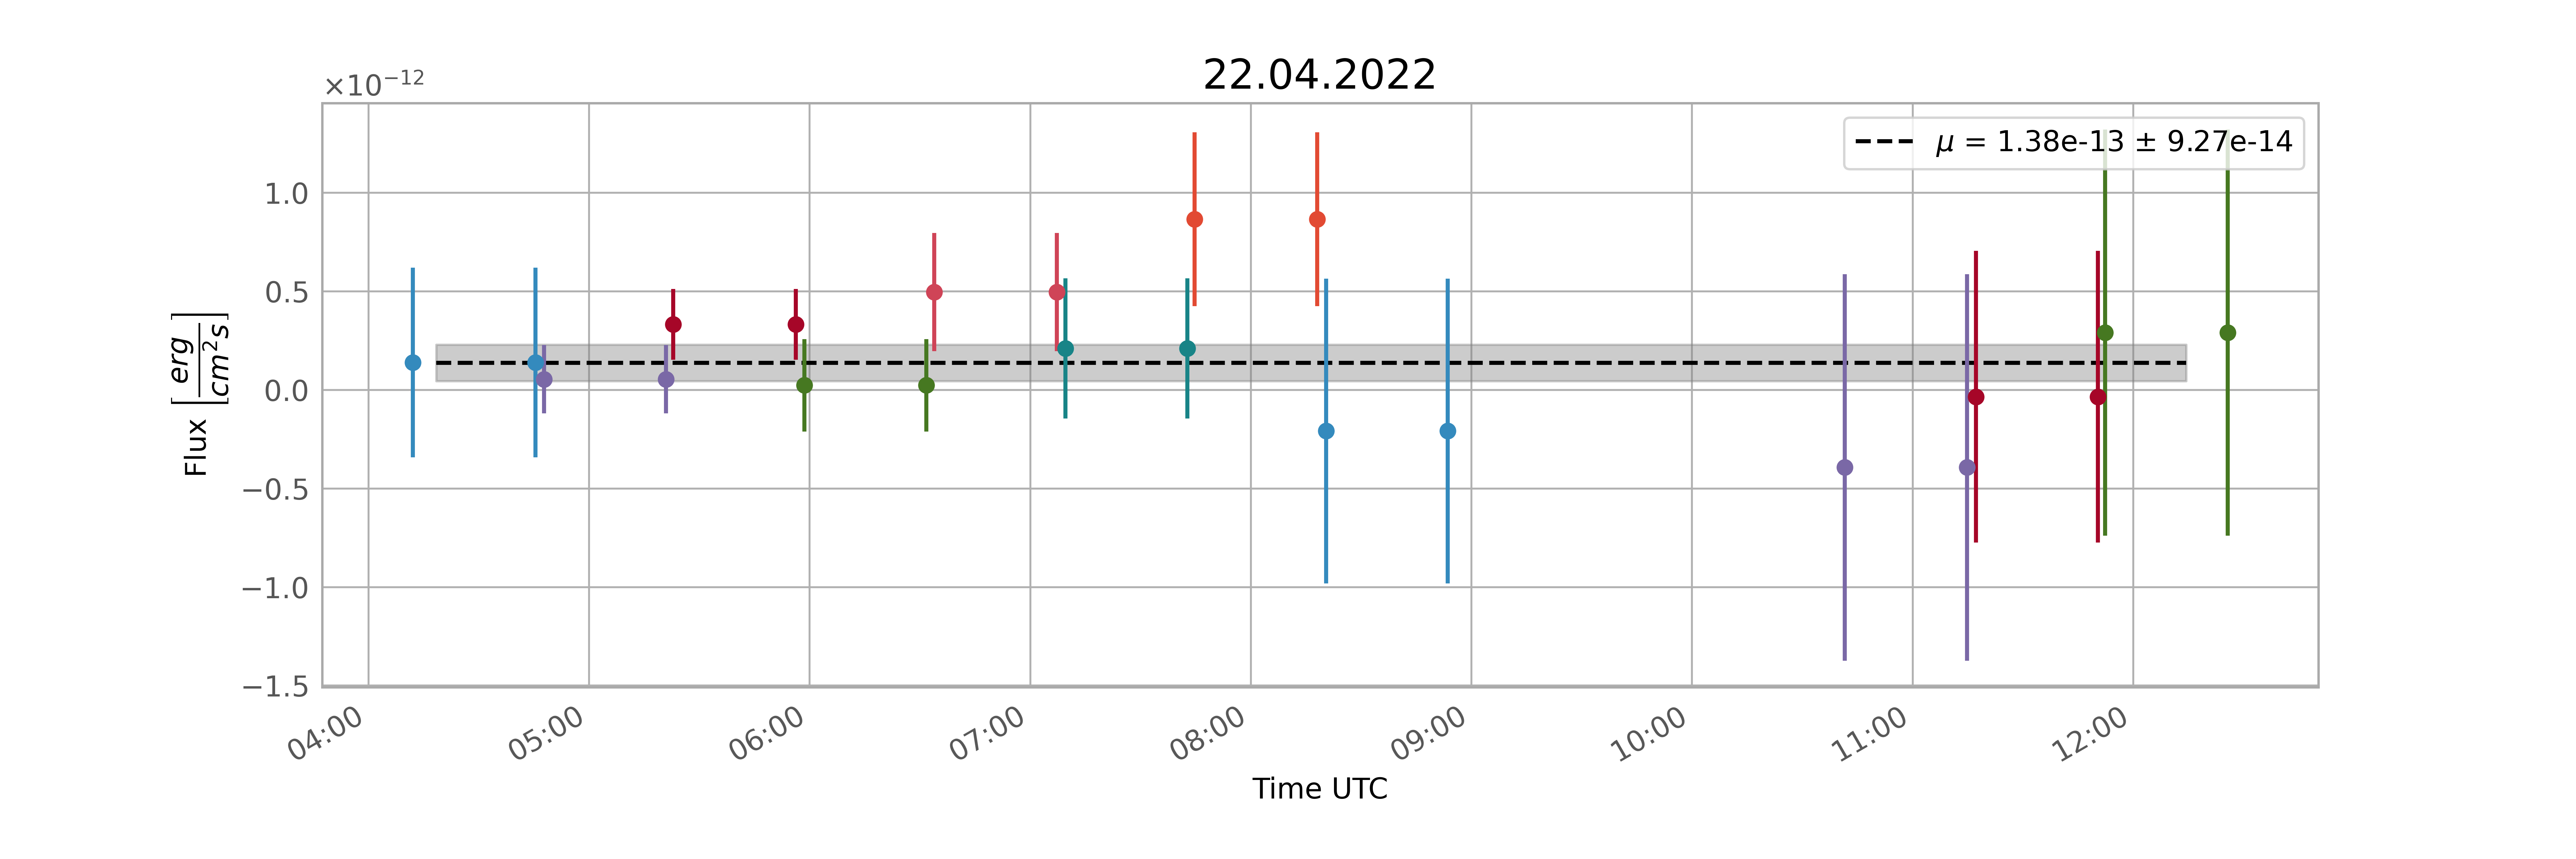
\includegraphics[width=\textwidth]{report/Figures/results/lc_2204_psf_const.png}
        \end{subfigure}
        \caption{For the 22.04.2022, from top to bottom: LC using the pixel value, the non constant PSF model and the constant PSF model.}
        \label{22_lc}
        \end{figure}
        

    \paragraph{24.04.2022 results}
    ???
        \begin{figure}[H]
        \centering
        \begin{subfigure}{\textwidth}
            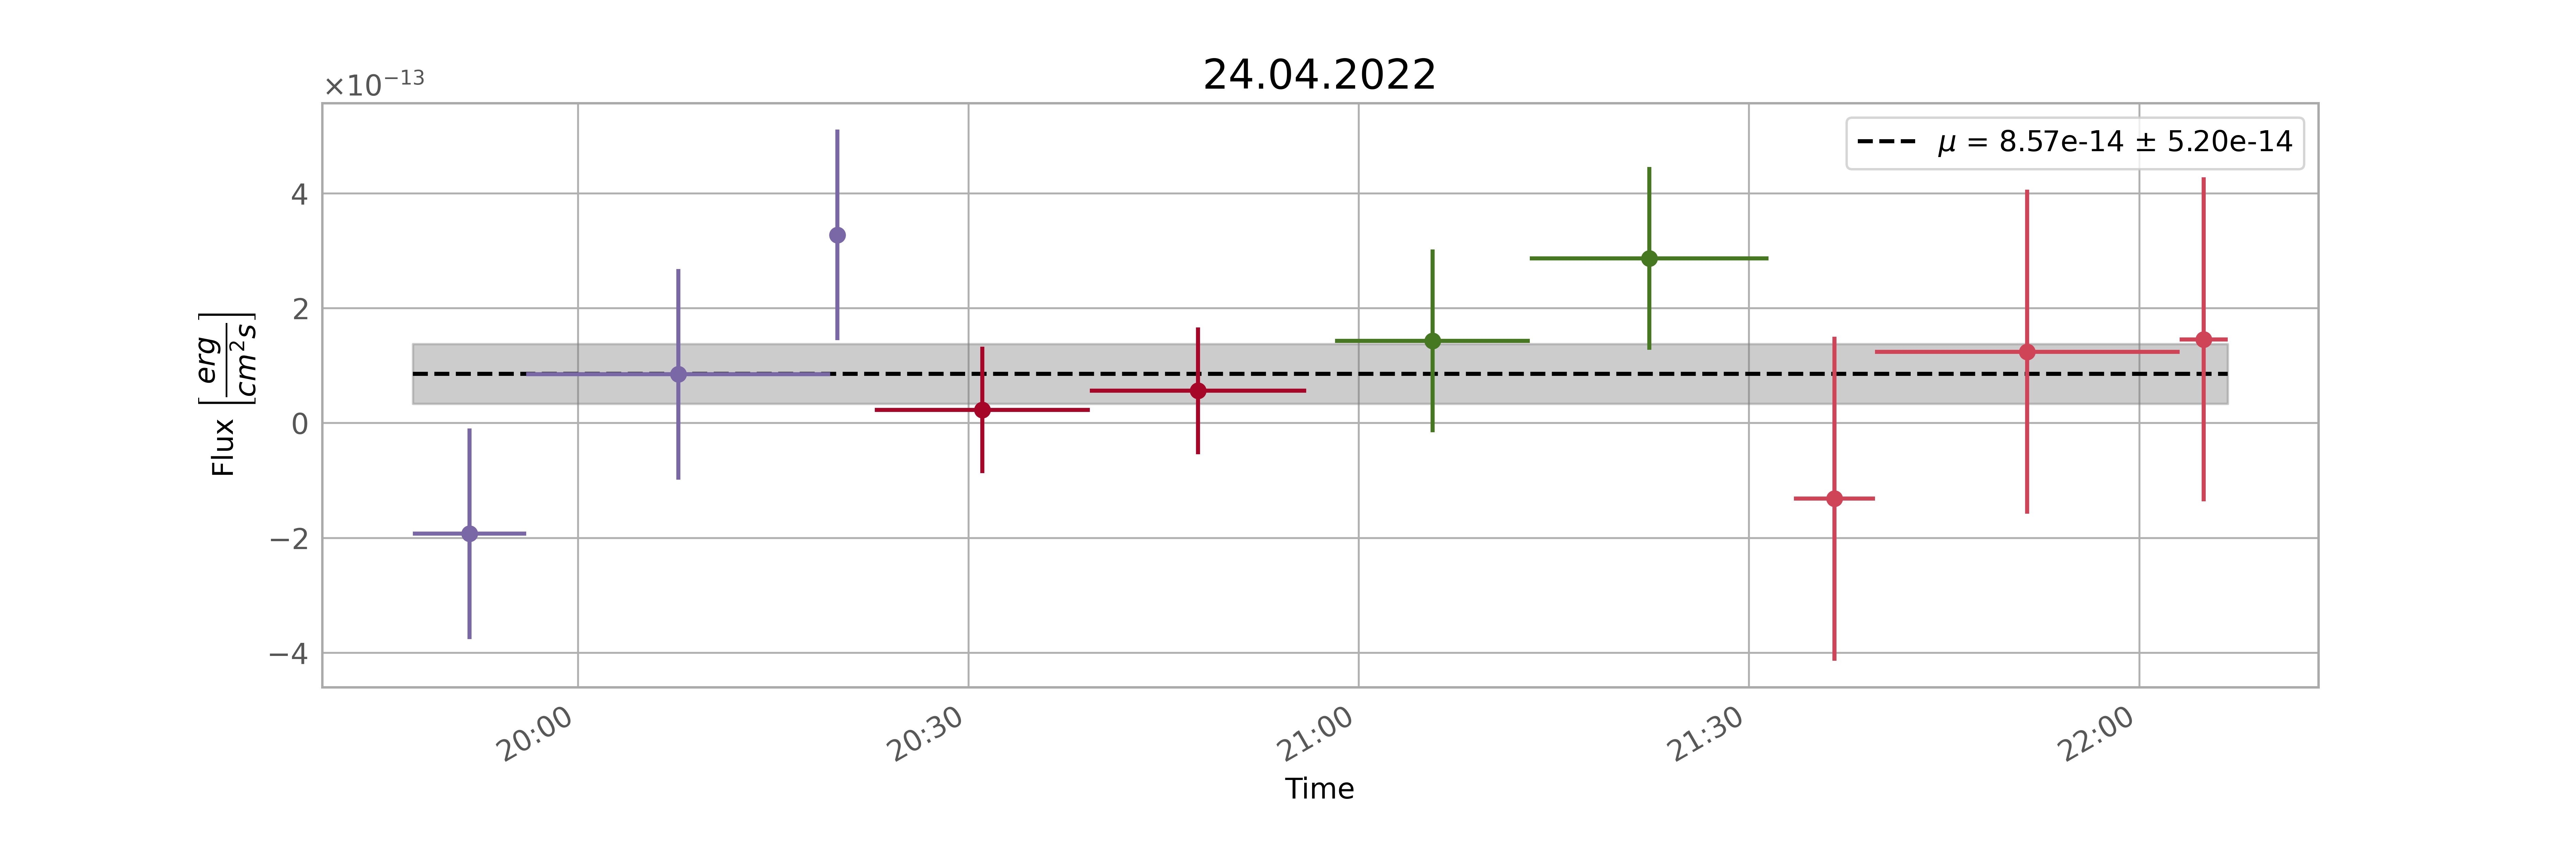
\includegraphics[width=\textwidth]{report/Figures/results/lc_2404.png}
        \end{subfigure}%
        \hspace{1em}
        \begin{subfigure}{\textwidth}
            \centering
            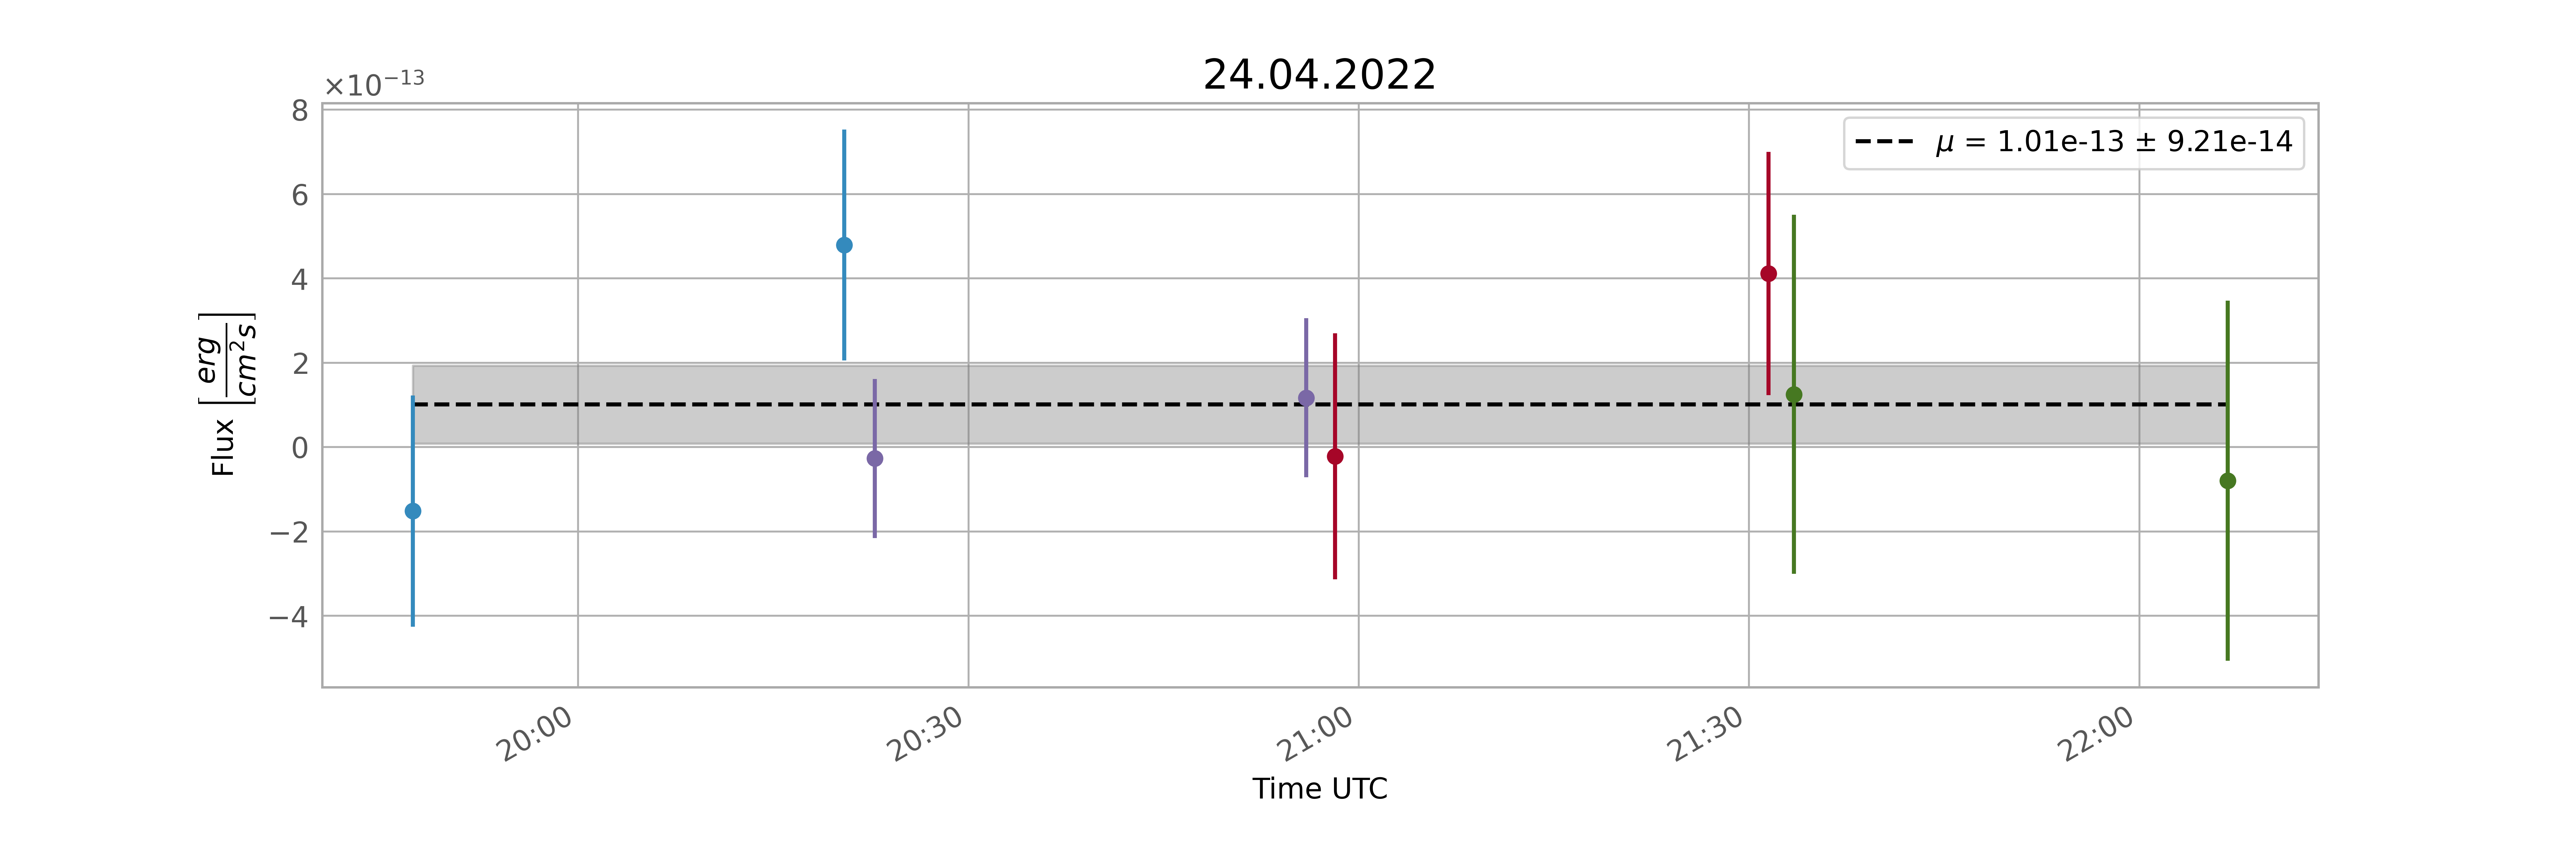
\includegraphics[width=\textwidth]{report/Figures/results/lc_2404_notconst.png}
        \end{subfigure}
        \hspace{1em}
        \begin{subfigure}{\textwidth}
            \centering
            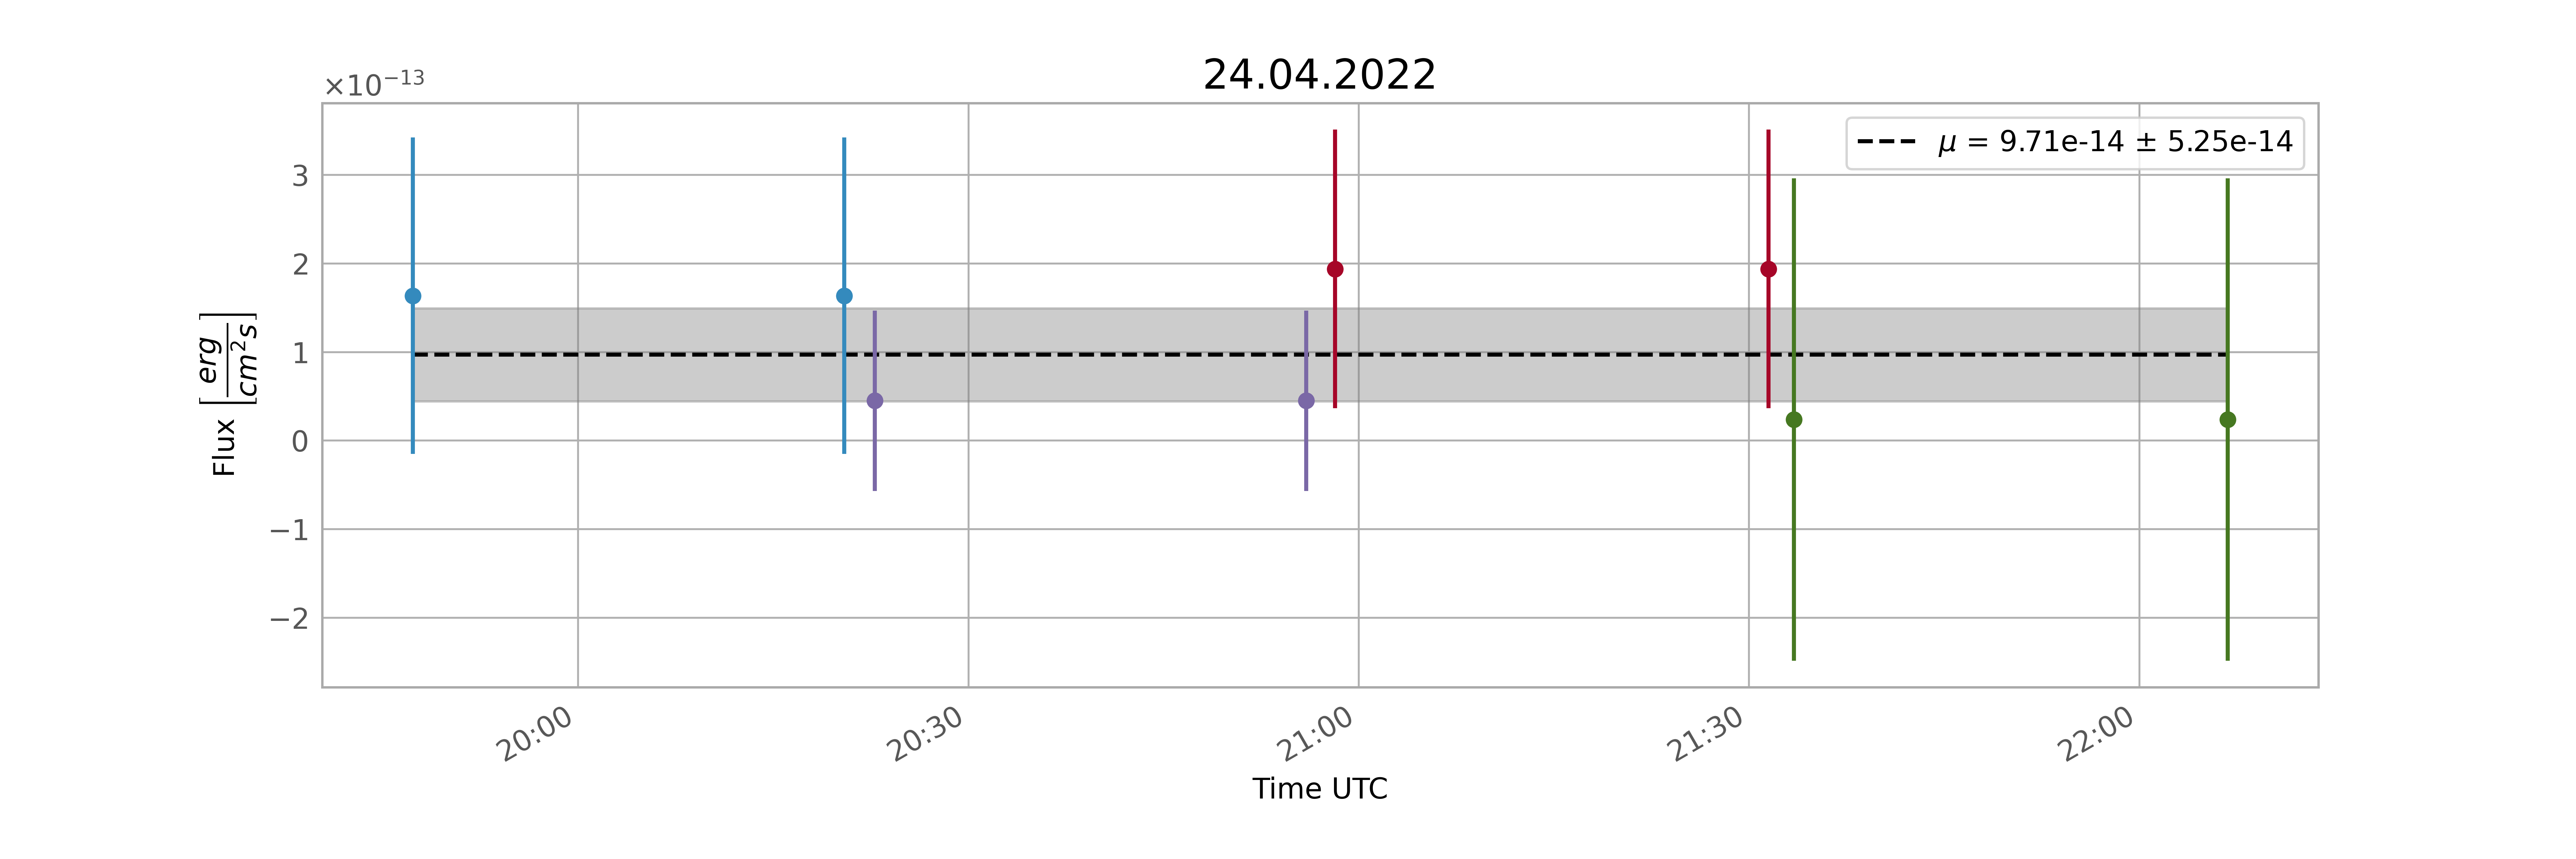
\includegraphics[width=\textwidth]{report/Figures/results/lc_2404_psf_const.png}
        \end{subfigure}
        \caption{For the 24.04.2022, from top to bottom: LC using the pixel value, the non constant PSF model and the constant PSF model.}
        \label{24_lc}
        \end{figure}

    \begin{figure}[H]
        \centering
        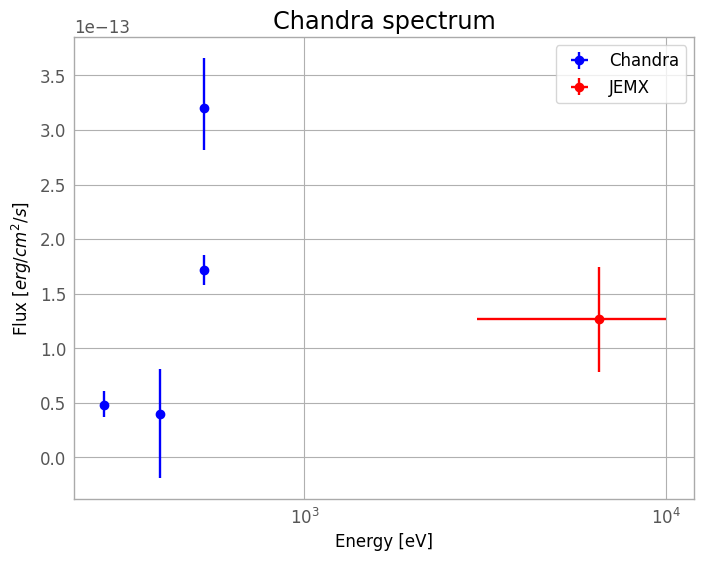
\includegraphics[width = 12cm]{report/Figures/results/spectra_comp.png}
        \caption{Comparison between the flux values obtained in ? and this study.}
        \label{comp_spec}
    \end{figure}
    
    \subsection{Concordance with solar flux variations}

    \begin{figure}[H]
        \centering
        \begin{subfigure}{\textwidth}
            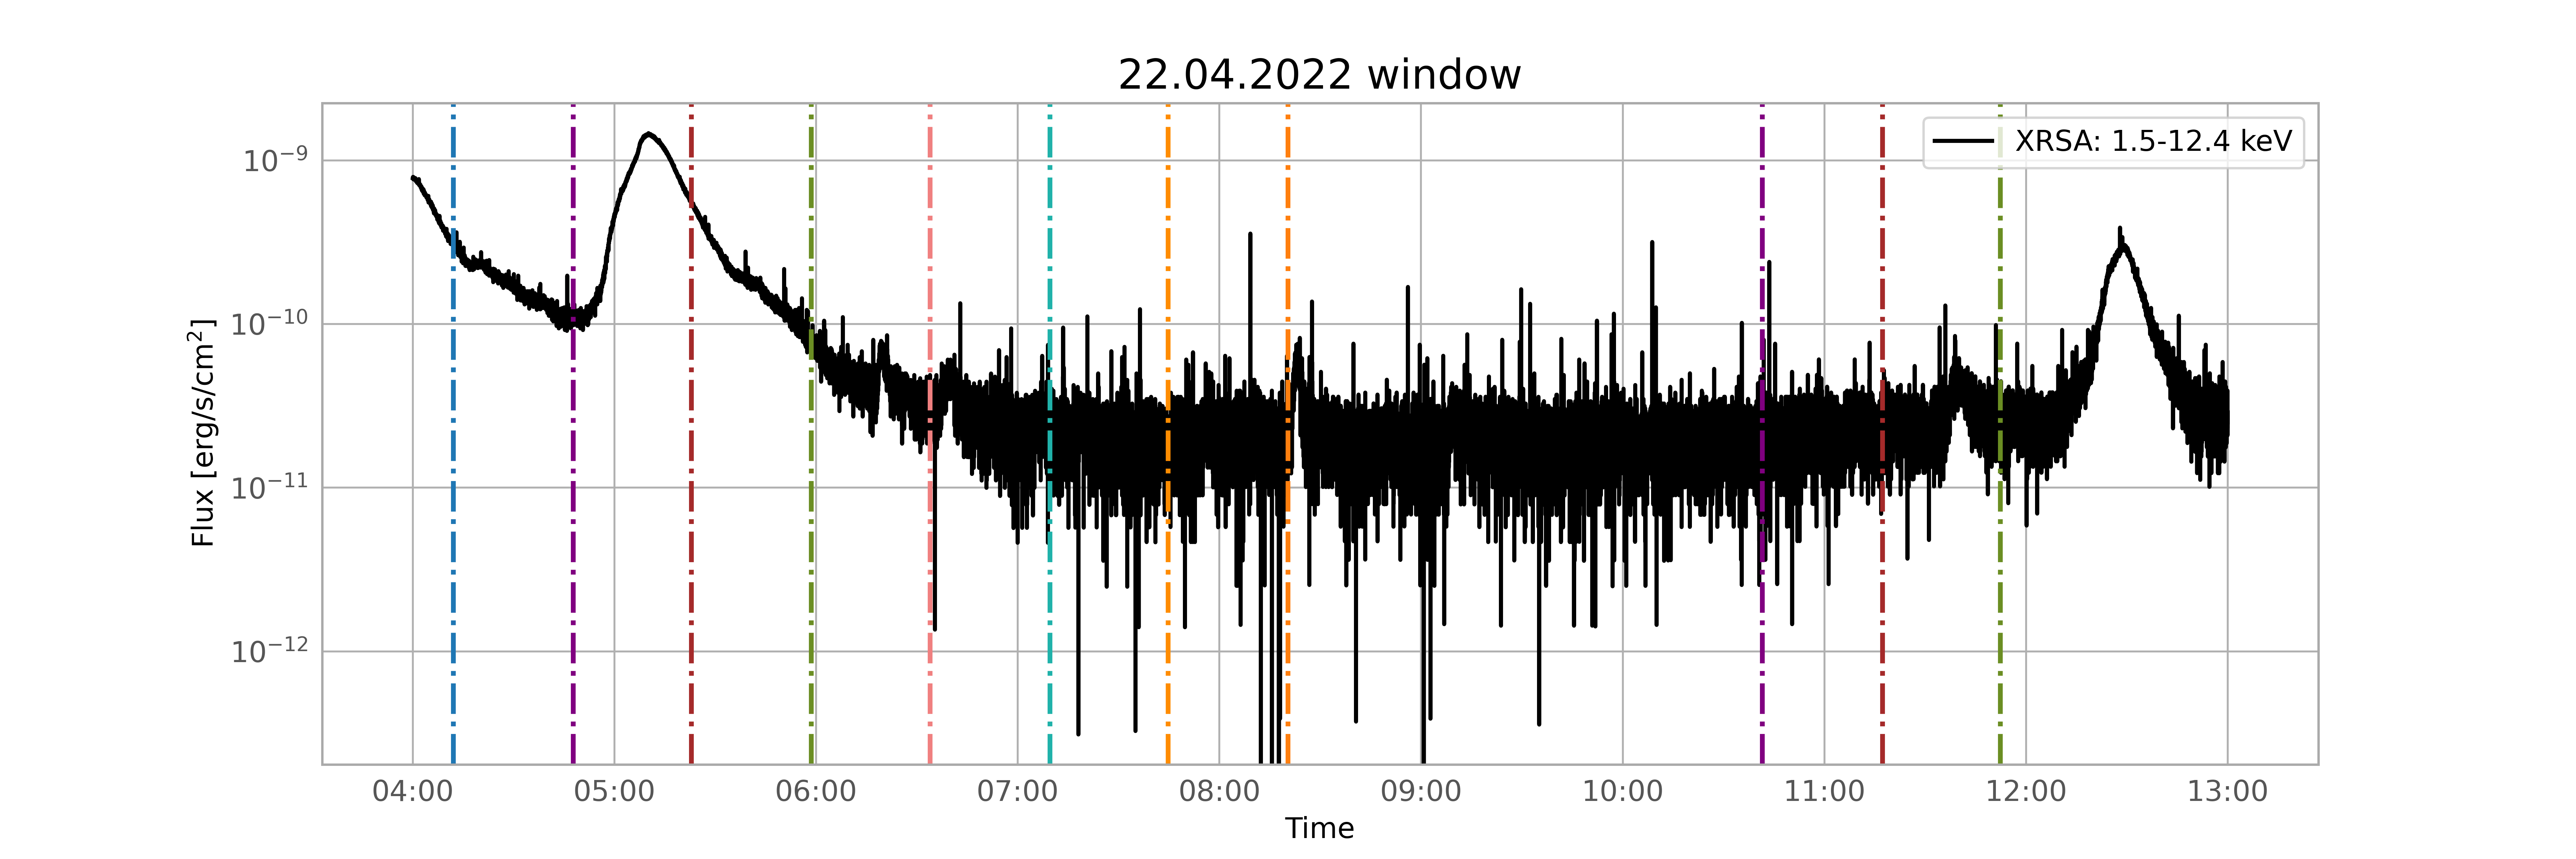
\includegraphics[width=\textwidth]{report/Figures/results/GOES_22.png}
        \end{subfigure}%
        \hspace{1em}
        \begin{subfigure}{\textwidth}
            \centering
            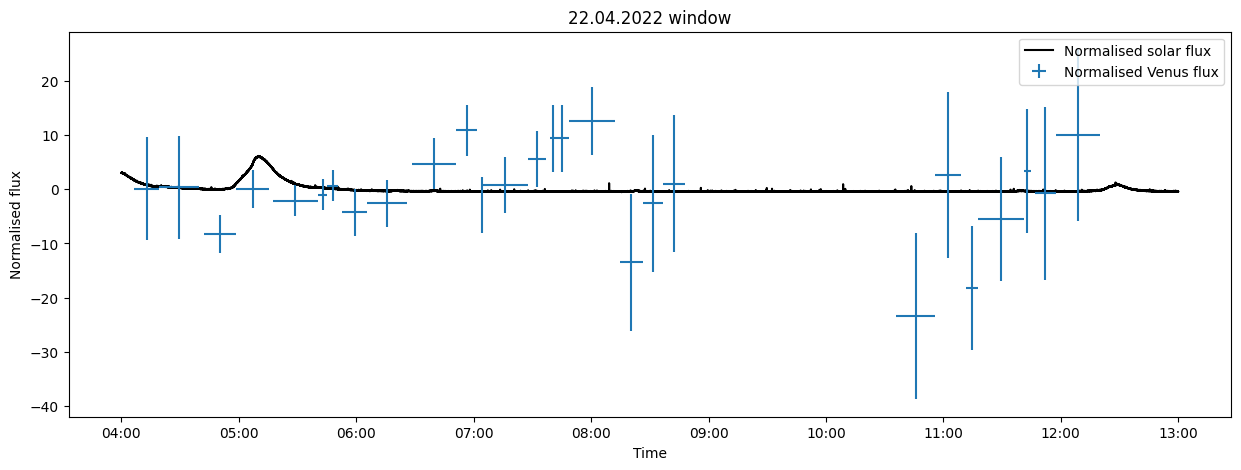
\includegraphics[width=\textwidth]{report/Figures/results/norm_22.png}
        \end{subfigure}
        \caption{Top: 22.04.2022 scws restricted view of the solar flux in the XRSA channel of GOES-16 overplotted with the times of the LC points.
        Bottom: Normalised solar and Venus fluxes plotted together. The data point times were corrected from light travel.}
        \label{goes22}
    \end{figure}

    \begin{figure}[H]
        \centering
        \begin{subfigure}{\textwidth}
            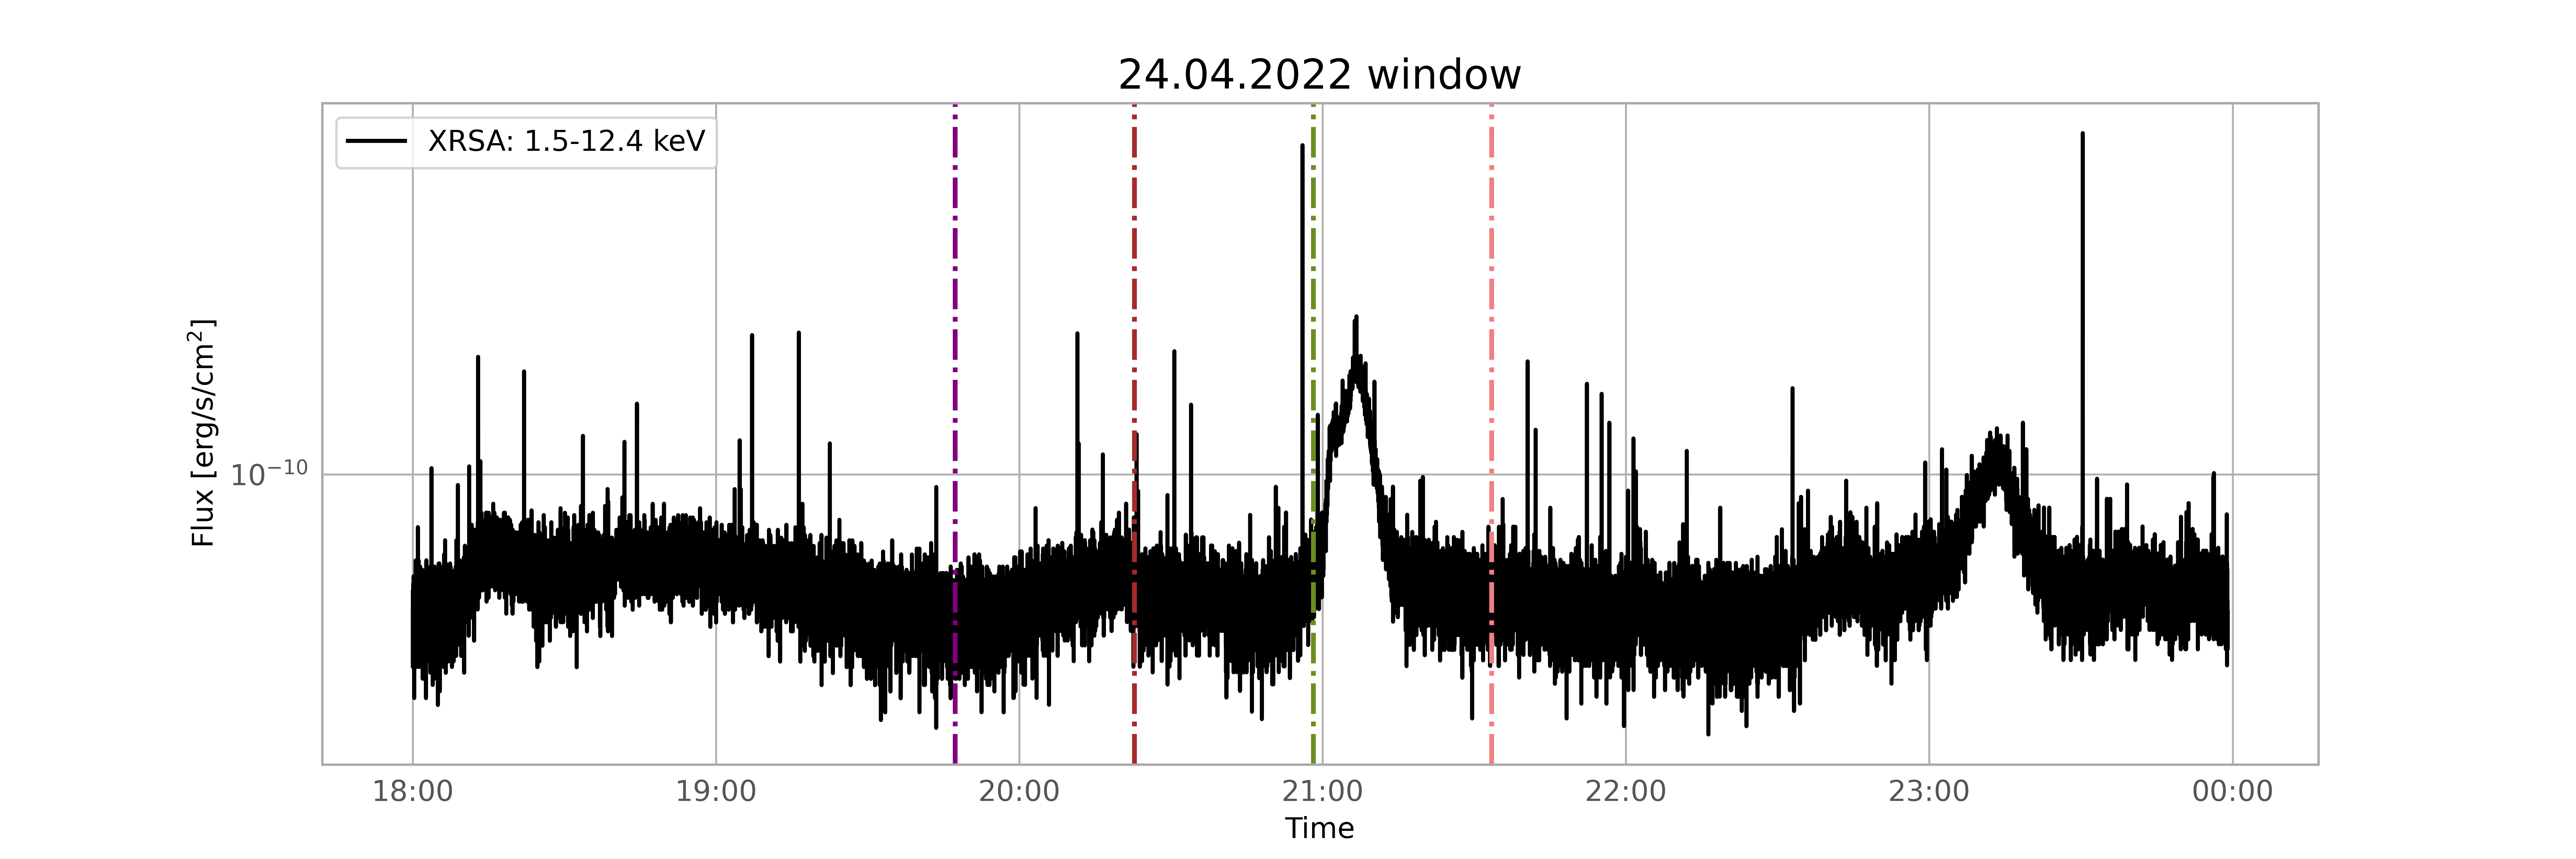
\includegraphics[width=\textwidth]{report/Figures/results/GOES_24.png}
        \end{subfigure}%
        \hspace{1em}
        \begin{subfigure}{\textwidth}
            \centering
            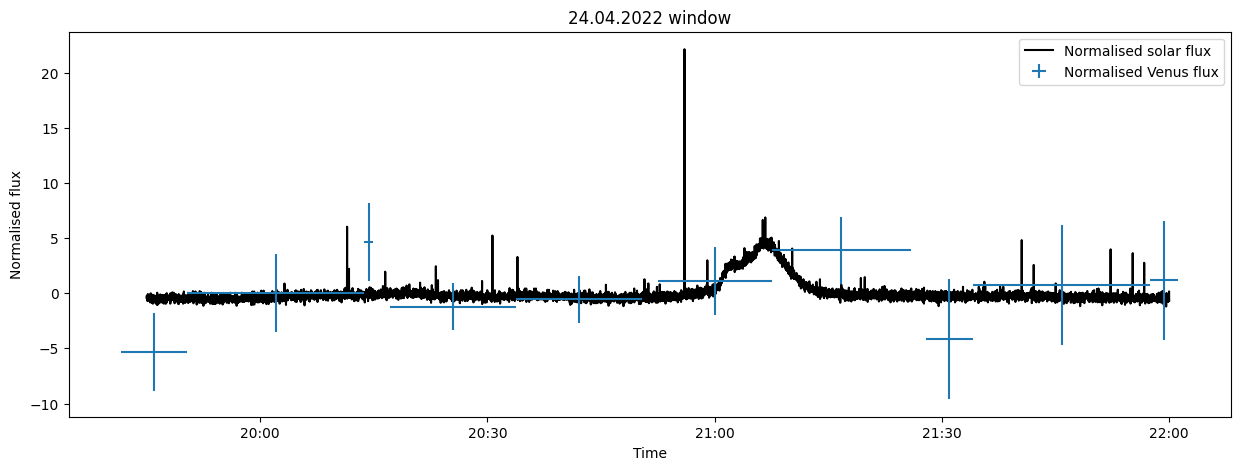
\includegraphics[width=\textwidth]{report/Figures/results/norm_24.png}
        \end{subfigure}
        \caption{Top: 24.04.2022 scws restricted view of the solar flux in the XRSA channel of GOES-16 overplotted with the times of the LC points.
        Bottom: Normalised solar and Venus fluxes plotted together. The data point times were corrected from light travel.}
        \label{goes_24}
    \end{figure}

    % talk about estimated energy deposited on venus too.
    
    \subsection{Solar events locations}
    blablabla

        \begin{figure}[H]
        \centering
        \begin{subfigure}{.47\textwidth}
            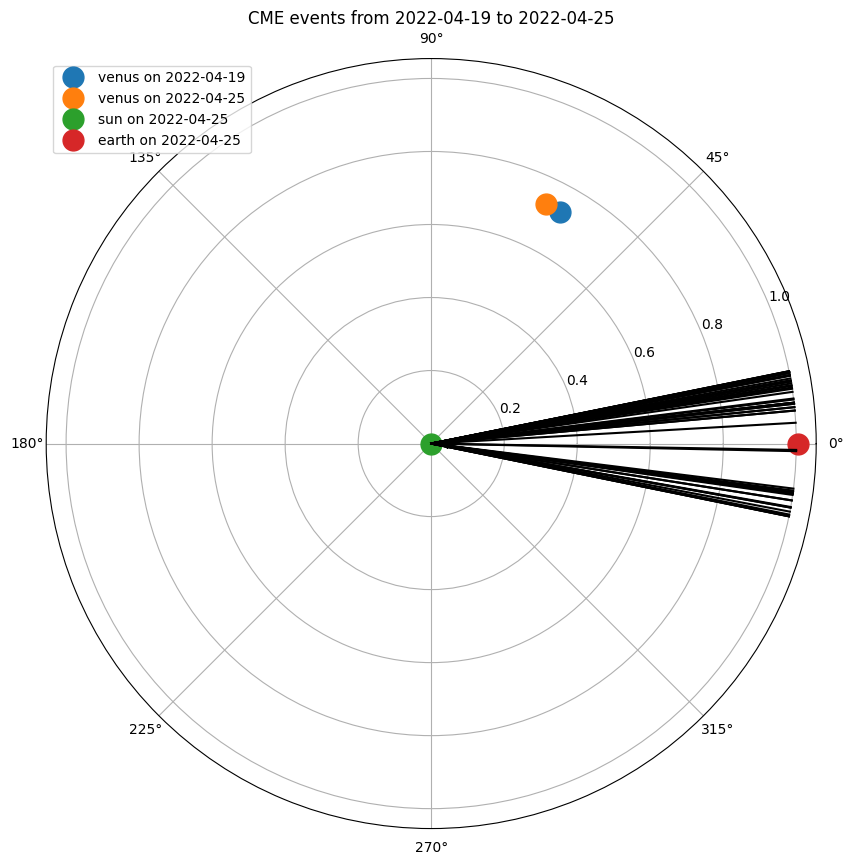
\includegraphics[width=\textwidth]{report/Figures/results/cme_loc.png}
        \end{subfigure}%
        \hspace{1em}
        \begin{subfigure}{.47\textwidth}
            \centering
            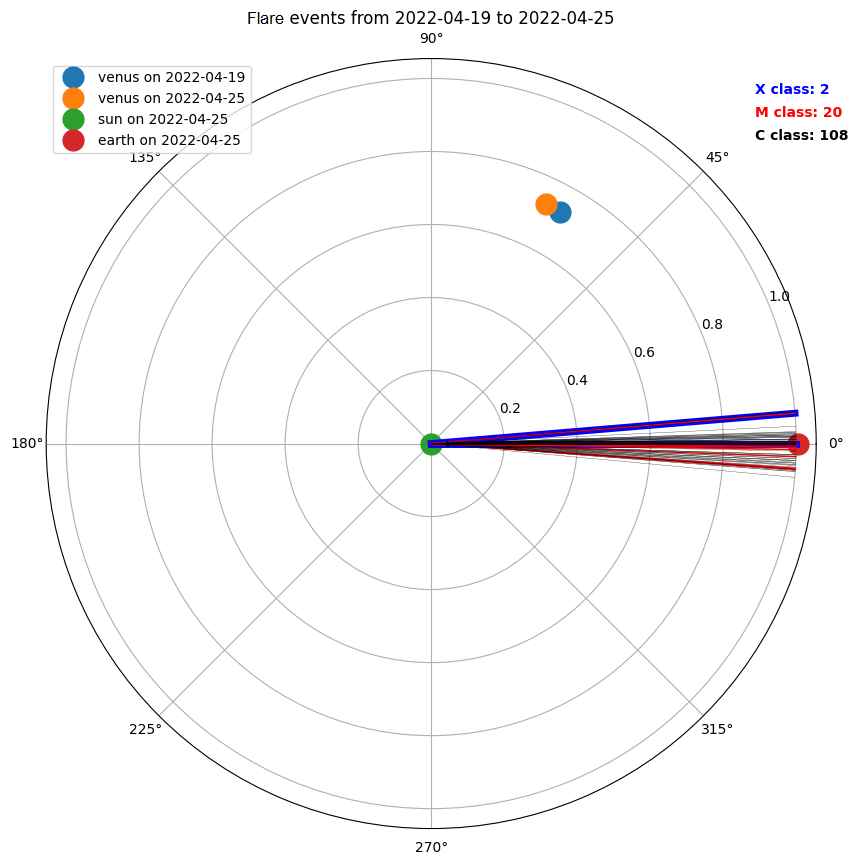
\includegraphics[width=\textwidth]{report/Figures/results/fl_loc.png}
        \end{subfigure}
        \caption{For the 19.04.2022 to 25.04.2022 period: (left) Propagation directions of all CMEs contained in the HEK. (right) Propagation directions of all flares contained in the HEK. The classes of the flares and numbers are indicated in colors.}
        \label{locator}
        \end{figure}

    \begin{figure}[H]
        \centering
        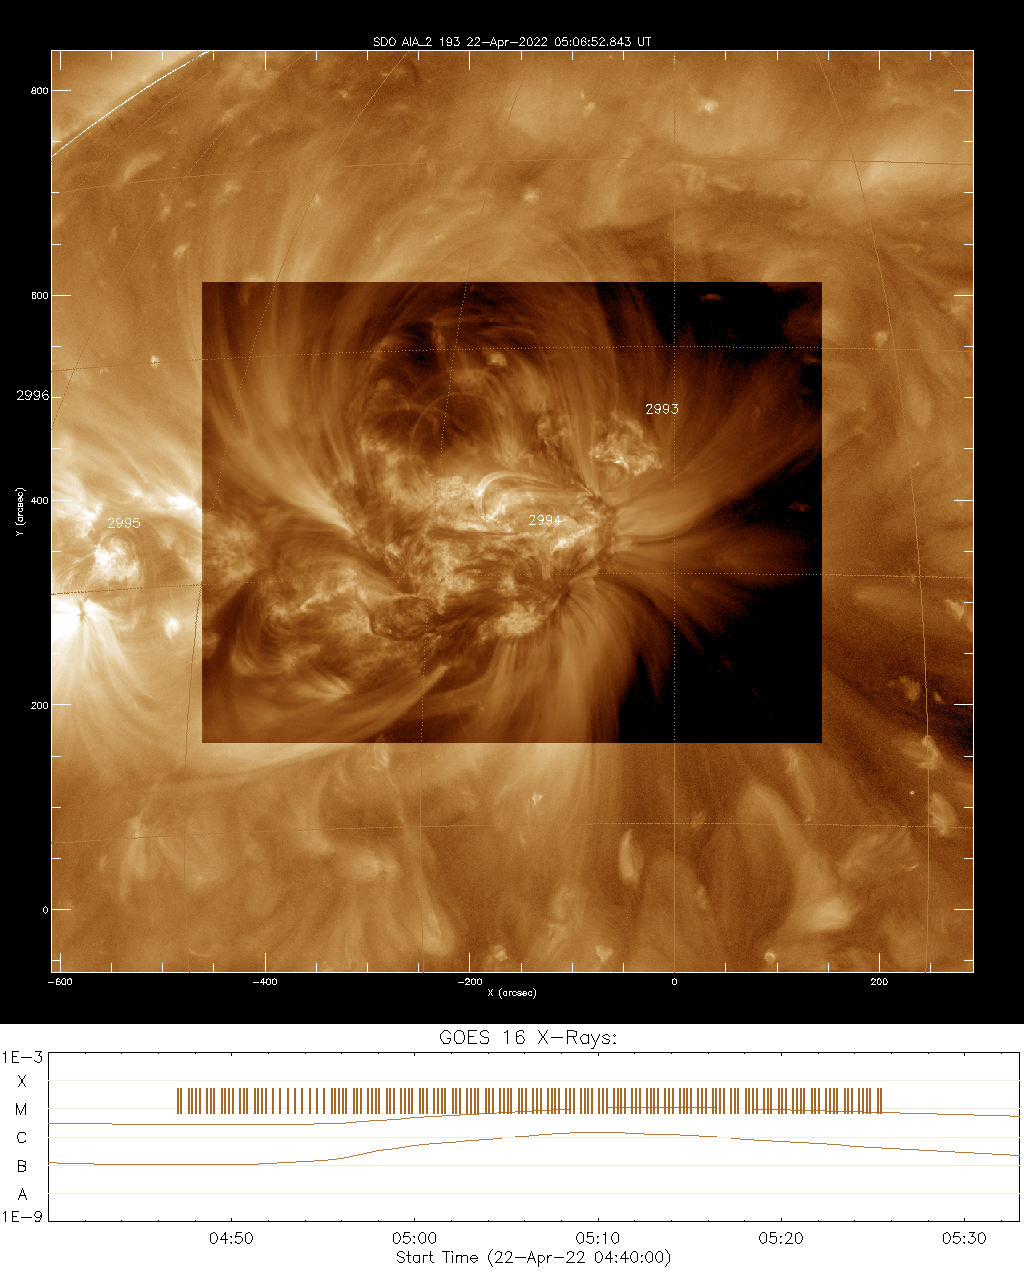
\includegraphics[width = 12cm]{report/Figures/results/aia_Mclass_2204.png}
        \caption{AIA image of the M1.1 class flare visible in the 22.04.2022 window.}
        \label{Mclass_flare}
    \end{figure}